\chapter{Project Idea}
\section{Task}
\label{sec:task}
The goal of this project is to create a reverse engineering lab. The students who take part in the labs should learn reversing step by step and get comfortable with tools like IDA Freeware, Radare2, Hopper or Ghidra. The labs should primarily be completed on either a Windows or a Linux system. \\
After a first analysis, the requirements for the reverse engineering labs and the exercises should be formulated. Afterwards the students should create 8 - 10 engineering labs. It is important that theres a common thread through all the labs. The participating students should start with easier examples and slowly solve more complex tasks. ASLR and DEP should be a part of the labs.

\section{Problem Domain}
To have an easy overview of the lab structure, a domain was created (see figure \ref{fig:mindmap}) at the beginning of the project. This ensured the projects goal is reached at the end. In addition to that, this mindmap is displayed in each of the labs to show the participating student which part of reverse engineering is taught.
\begin{figure}[H]
    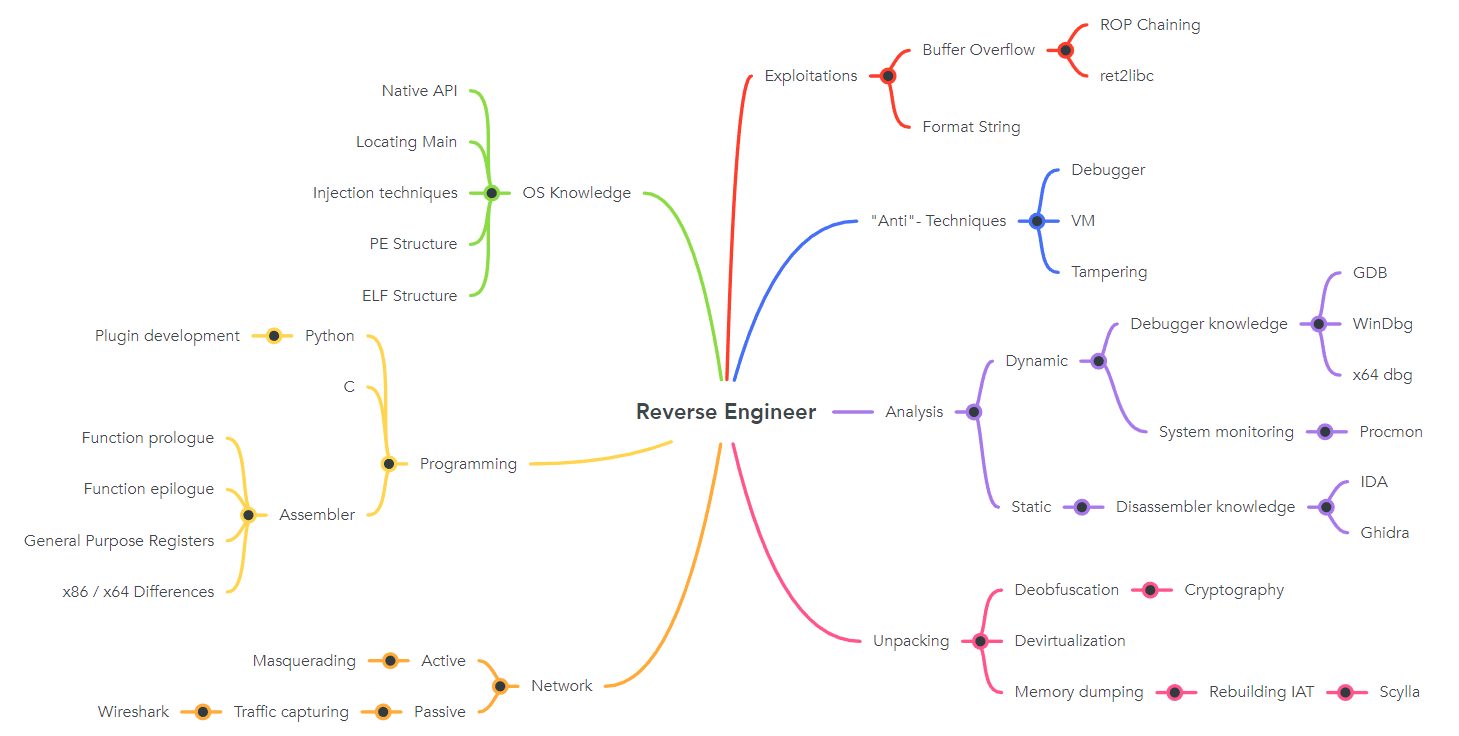
\includegraphics[width=\linewidth, center]{resources/RE_Domain_Light.png}
    \caption{Mindmap of the knowledge a Reverse Engineer needs.}
    \label{fig:mindmap}
\end{figure}

\section{Learning Concepts}
Before each lab is created a proof of concept (POC) has to be defined. These concepts contain the information which part of the problem domain in figure \ref{fig:mindmap} is taught, how the lab is structured and what the teacher has to explain beforehand. The lab names and content were defined in a way that the student solving them has a clear thread to follow and goes from easier to harder exercises. \\
To assure the labs could be completed as planned it is assumed that the students have a basic knowledge in assembly language (ASM), Python and C. Since ASM is the most important language to understand the fundamental structure of a binary, a lab for refreshing this knowledge is planned.\\
The lab titles and content changed over the time of the project and the final scope of the labs differs from the one at the beginning. The final list is shown in table \ref{tab:labs}. 

\begin{center}
    \begin{table}[H]
        \centering
        \begin{tabular}{ |p{4.1cm}|p{10cm}| } 
            \hline
                Topic & 
                Description \\ [0.5ex] 
            \hline
            \hline
                Tutorial for the tools: GDB & Introduction into GDB and its tools \\
            \hline
                Tutorial for the tools: x64dbg & Introduction into x64dbg and how to navigate the GUI \\
            \hline
                Tutorial for the tools: IDA Freeware & Introduction into IDA Freeware and how to navigate the GUI \\
            \hline
                Refresher & 
                Give the students some little refreshing on the key topics (Assembly)  \\ 
            \hline
                Static Debugging & 
                Given a simple C file, students compile it and try to find a key (Find Main function) \\ 
            \hline
                Dynamic Debugging & 
                Given a simple C file, students compile it and try to find a key (go more into GDB / x64) \\ 
            \hline
                First RE attempts & 
                Given simple files compiled in several languages (PY, C\#, C++) get flag \\ 
            \hline
                Remote Login  & 
                Inspecting binanry locally and using RE to gain access to a remote docker-container \\
            \hline
                Pwntools & 
                Exploiting a through RE found vulnerability with pwntools \\
            \hline
                AES Encryption & 
                Not only finding out the password but writing a keygen for the program \\
            \hline
                Patching a Binary & 
                Introduce new native API funcs / techniques like stack strings \\
            \hline
        \end{tabular}
        \caption{Overview of all the Labs.}
        \label{tab:labs}
    \end{table}
\end{center}
